
% ---------- Titelblad Masterproef Faculteit Wetenschappen -----------
% Dit document is opgesteld voor compilatie met pdflatex.  Indien je
% wilt compileren met latex naar dvi/ps, dien je de figuren naar
% (e)ps-formaat om te zetten.
%                           -- december 2012
% -------------------------------------------------------------------
\RequirePackage{fix-cm}
\documentclass[12pt,a4paper,oneside]{article}

% --------------------- In te laden pakketten -----------------------
% Deze kan je eventueel toevoegen aan de pakketten die je al inlaadt
% als je dit titelblad integreert met de rest van thesis.
% -------------------------------------------------------------------
\usepackage{graphicx,xcolor,textpos}
\usepackage{helvet}

% -------------------- Pagina-instellingen --------------------------
% Indien je deze wijzigt, zal het titelblad ook wijzigen.  Dit dien je
% dan manueel aan te passen.
% --------------------------------------------------------------------

\topmargin -10mm
\textwidth 160truemm
\textheight 240truemm
\oddsidemargin 0mm
\evensidemargin 0mm

% ------------------- textpos-instellingen ---------------------------
% Enkele andere instellingen voor het voorblad.
% --------------------------------------------------------------------

\definecolor{green}{RGB}{172,196,0}
\definecolor{bluetitle}{RGB}{29,141,176}
\definecolor{blueaff}{RGB}{0,0,128}
\definecolor{blueline}{RGB}{82,189,236}
\setlength{\TPHorizModule}{1mm}
\setlength{\TPVertModule}{1mm}



%----------------------- Custom stuff -------------------------------

\graphicspath{./}
\usepackage{makeidx}
\index{hoofd}
\makeindex
\usepackage{amsmath}
\usepackage[english]{babel}
\usepackage{hyperref}
\usepackage{listings}
\usepackage{eurosym}


%------------------------ Plot packages ----------------------------
\usepackage{tikz}
\usepackage{pgfplots}
\usepackage{pgf}
\usepackage{units}
\usepackage{metalogo}
\usepackage{graphicx}
\usepackage{caption}
\usepackage{subcaption}
\usepackage{standalone}


%----------------------Title etc----------------------------------
\title{Non linear Systems: Laser Model Analysis}
\author{Moritz Wolter}
\date{\today}


% --------------------------------------------------------------------

\begin{document}

\title{Exercise 6 Pattern formation}
\author{Moritz Wolter}

\maketitle

\section{The Brusselator}
\begin{align}
u_t &= D_u u_{xx} + A - (B + 1)u + u^2 v, \\
v_t &= D_v v_{xx} + Bu - u^2 .
\end{align}
The above equations describe molecule concentrations during a coupled reaction. They are known to exhibit patterns.  

\section{Stability of the steady state}
At the steady state $u_t = v_t = u_{xx} = v_{xx} = 0$. Thus following equations remain:
\begin{align}
0 &= A - (B + 1)u + u^2v, \\
0 &= u(B - uv). \\
\end{align}
From which $u_0 = A$ and $v_0 = B/A$ is deduced. Considering the linearized system evaluated at $u_0$,$v_0$ in Matrix form:
\begin{align}
\begin{pmatrix}
u_t \\ v_t
\end{pmatrix} =
\begin{pmatrix}
D_u u_{xx} \\ D_v v_{xx}
\end{pmatrix} +
\underbrace{\begin{pmatrix}
B-1 & A^2 \\
-B & -A^2
\end{pmatrix}}_\text{Jacobian evaluated at $(u_0,v_0)$}
\begin{pmatrix}
u \\ v
\end{pmatrix}. 
\label{eq:lin} 
\end{align}
From the Jacobian above trace and determinant of the ordinariy differential subsystem can be read off, $\tau_{ode} = B - 1 - A^2$ and $\triangle_{ode} = A^2$.
Using $\begin{pmatrix} u & v \end{pmatrix}^T = \begin{pmatrix} u_1 & v_1 \end{pmatrix}^T \cdot \exp(\lambda t + ikx)$ leads to:
\begin{align}
u_{xx} &= (ik)^2 u_1 \exp(s t + ikx) = -k^2u \\
u_{yy} &= (ik)^2 v_1 \exp(s t + ikx) = -k^2v
\end{align}
When substituting this into the linearized equation~\ref{eq:lin}. The expression:
\begin{equation}
\begin{pmatrix}
u_t \\ v_t
\end{pmatrix} =
\begin{pmatrix}
(B - 1)-k^2 D_u & A^2 \\
-B & -A^2-k^2 D_v
\end{pmatrix}
\begin{pmatrix}
u \\ v
\end{pmatrix}.
\end{equation}
The new matrix above has trace $\tau$ and determinant $\triangle$:
\begin{align}
\tau &= B - 1 - A^2 - k^2(D_u + D_v) \\
\triangle &= [(B-1) - k^2 D_u ][-A^2 - k^2D_v] + BA^2 \\
		  &= A^2 - BA^2 + A^2k^2D_u + k^2D_vB - k^2 D_v + k^2 D_u D_v + BA^2 \\
		  &= A^2 + k^2(A^2 D_u + (1 - B)D_v ) + k^4 D_u D_v.
\end{align}
Now linear algebra has a nice relationship for the eigenvalues:
\begin{equation}
\lambda_\pm = \frac{1}{2}(\tau \pm \sqrt{\tau^2 - 4\triangle}).
\end{equation}
\section{Turing instability}
Turing instability can occur when the ordinary differential and the partial differential part of the system work against each other. Or in other terms it instability is requires:
\begin{align}
\tau_{ode} < 0 \wedge \triangle_{ode} > 0 \\
(\tau_{pde} > 0 \wedge \triangle_{pde} > 0) \vee \triangle_{pde} < 0.
\end{align}
Where the subscripted $\tau_{ode}$ and $\triangle_{ode}$ denote trace and determinant of the ordinary differential system and $\tau_{pde}$ and $\triangle_{pde}$ trace and determinant of the partial differential part. When real eigenvalues of the partial differential subsystem change sign, the onset of Turing instability is observed. That is because the determinant which is the product of the two eigenvalues will change it's sign if any of the eigenvalues do. If both pde system eigenvalues change sign with respect to the ode system, $\tau_{pde}$ changes it's sign instead of $\triangle_{pde}$.

Using the conditions outlined above a critical value for $B$ may be computed, looking at the inequalities for the ordinary part:
\begin{align}
\tau_{ode} &= B - 1 - A^2 < 0 \Leftrightarrow B < 1 + A^2 \\
\triangle_{ode} &= A^2 > 0.
\end{align}
The two inequalities have to be respected, when creating an turing unstable Brusselator. Starting from $\triangle_{pde} = 0$. A critical value for an increasing B is sought after in the upcoming part:
\begin{align}
0 &= A^2 + k^2 (A^2 D_u + (1 - B)D_v) + k^4D_u D_v \\
B &= \frac{A^2 D_u}{D_v} + 1 + \frac{A^2}{k^2 D_v} + k^2 D_u. 
\label{eq:B}
\end{align}
However to evaluate the expression above a value for the variable $k$ is required. As the goal of this train of thought is to find the smallest $B$ for which instability occurs, $k$ hast to be chosen such that it minimizes $B$. This can be done by solving $\frac{dB}{dk} = 0$ and later checking that $\frac{d^2 B}{dk^2} > 0$ to verify a minimum. The first derivative is given by:
\begin{align}
0 &= -\frac{2 A^2}{k^3 D_v} + 2kD_u \\
\Leftrightarrow 2A^2 &= 2k^4 D_u D_v \\
\Leftrightarrow k^4 &= \frac{A^2}{D_u D_v} \\
\Leftrightarrow k_T &= (\frac{A^2}{D_u D_v})^\frac{1}{4}.
\end{align}
The second derivative is described by:
\begin{equation}
\frac{d^2B}{dk^2} =\frac{6 A^2}{k^4 D_v} + 2 D_u
\label{eq:secDiv}
\end{equation}
Substituting $k_T$ into \ref{eq:secDiv} yields:
\begin{align}
\frac{d^2B}{dk^2}(k_T) = \frac{6A^2}{\frac{A^2}{D_u D_v} D_v} + 2D_u \\
= 8 D_u > 0 
\end{align}
Which proves that $k_T$ indeed is at a minimum of $B(k)$. Thus $k_T$ is now substituted into equation~\ref{eq:B} to find $B_T$:
\begin{align}
B &= 1 + \frac{A^2}{\frac{A^2}{D_u D_v}^\frac{1}{2} D_v} + \frac{A^2D_u}{D_v} + \frac{A^2}{D_u D_v}^\frac{1}{2} D_u \\
 &= 1 + \frac{A \sqrt{D_u D_v}}{D_v} + \frac{A^2 D_u}{D_v} + \frac{A D_u}{\sqrt{D_u D_v}} \\
 &= 1 + \frac{2AD_u D_v}{D_v \sqrt{D_u D_v}} + \frac{A^2 D_u \sqrt{D_u D_v}}{Dv \sqrt{D_u D_v}} \\
 &= 1 + 2A \sqrt{\frac{D_u^2}{D_u D_v}} + A^2\frac{D_u}{D_v} \\
\Leftrightarrow B_T &= (1 + A\eta)^2.
\end{align}
With $\eta = \sqrt{\frac{D_u}{D_v}}$ the critical value for $B_T$ has been found. 

\section{Alan vs Eberhard}
In this section the possibility of a Hopf-bifurcation occuring before Turing instability will be explored. Neglecting the diffusion terms trace and determinant are given by:
\begin{align}
\tau_{ode} = B - 1 - A^2 \\
\triangle_{ode} = A^2
\end{align}
A Hopf bifurcation happens when imaginary eigenvalues $\lambda_\pm = \frac{1}{2}(\tau \pm \sqrt{\tau^2 - 4\triangle})$ cross the real axis. Which happens when $\tau = 0$, if the determinant if positive. Thus at $B_H = (1 + A^2)$ the system exhibits a Hopf bifurcation as $\triangle_{ode}$ is positive. However Turing instability will occur first if:
\begin{align}
B_t < B_h \Leftrightarrow (1 + A\eta)^2 < (1 + A^2) \Leftrightarrow 1 + A\eta < \sqrt{1 + A^2} \Leftrightarrow \eta < \frac{\sqrt{1 + A^2} - 1}{A}.
\end{align}
\section{Numerical simulations}
If $B$ is chosen such that $B > B_T = 6.7132$ if $A = 4.5,D_u = 1 \text{ and } D_v = 8$, various patterns emerge as shown in figure~\ref{fig:Brussl1} . A simulation with \texttt{200} instead of \texttt{100} grid points for the same input parameters is shown in figure~\ref{fig:Brussl3}. If $B$ is increased further it is observed that the concentration of $u$ drops on average, which manifests in expanding blue dots, which show low concentration. At one point the dots merge and form blue lines, which can be seen in figure~\ref{fig:Brussl2}.

\begin{figure}
\centering
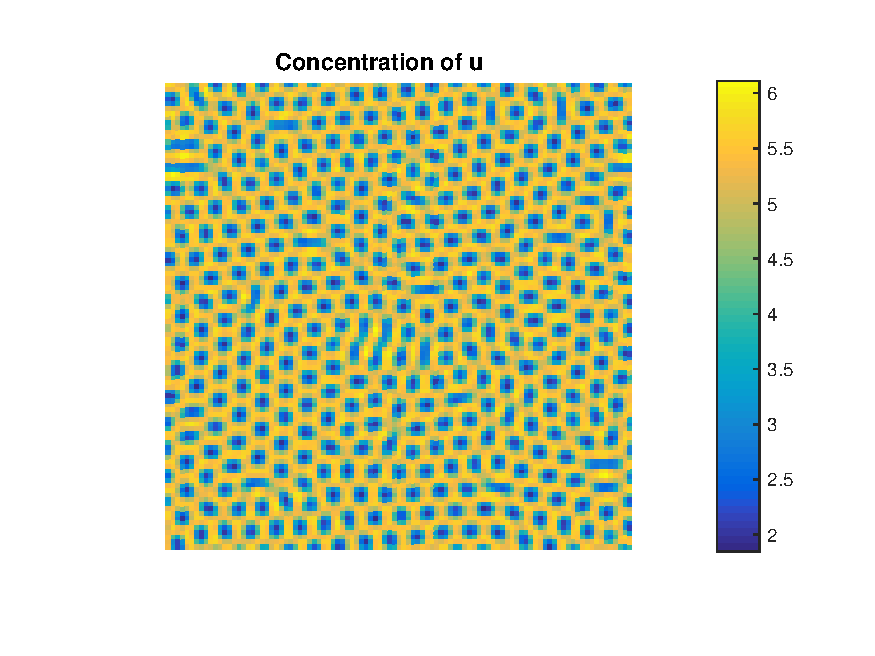
\includegraphics[scale = 0.9]{./plots/cua4p5b7.pdf}
%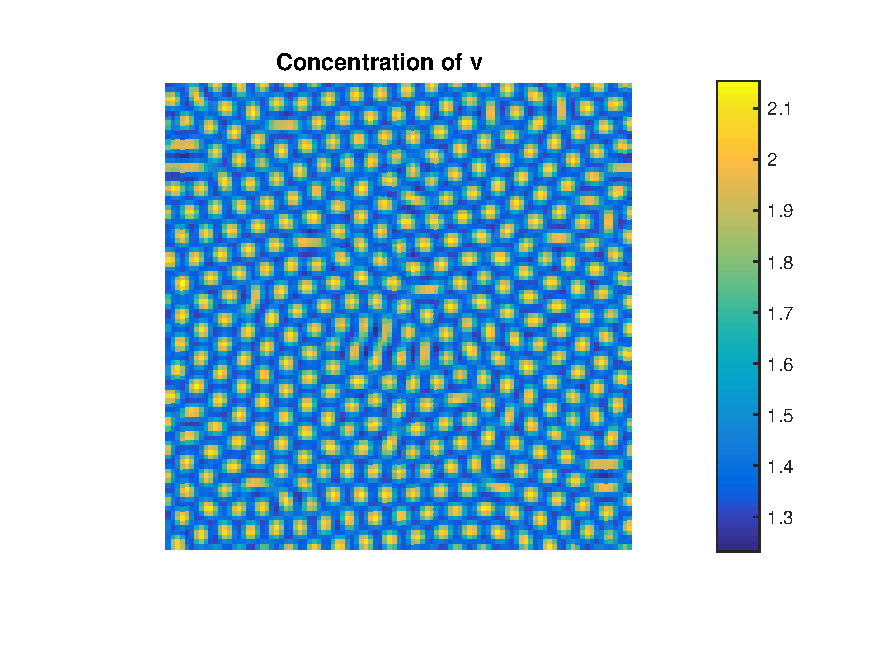
\includegraphics[scale = 0.5]{./plots/cva4p5b7.pdf}
\caption{Brusselator simulation output for $a=4.5,b=7,D_u=1,D_v=8$.}
\label{fig:Brussl1}
\end{figure}
\begin{figure}
\centering
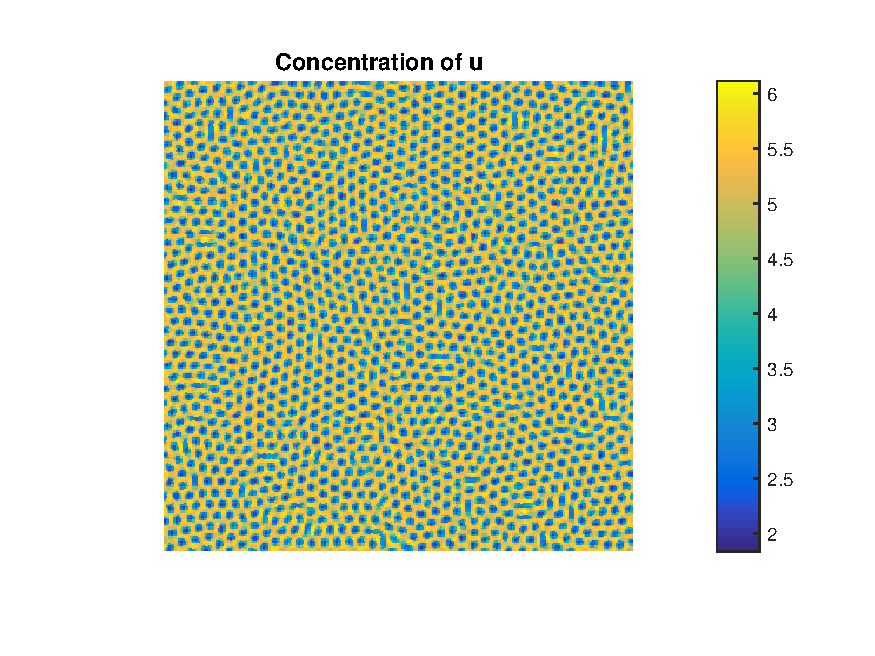
\includegraphics[scale = 0.9]{./plots/cua4p5b7g200.pdf}
\caption{Brusselator simulation output for $a=4.5,b=7,D_u=1,D_v=8$. With twice as many grid points.}
\label{fig:Brussl3}
\end{figure}
\begin{figure}
\centering
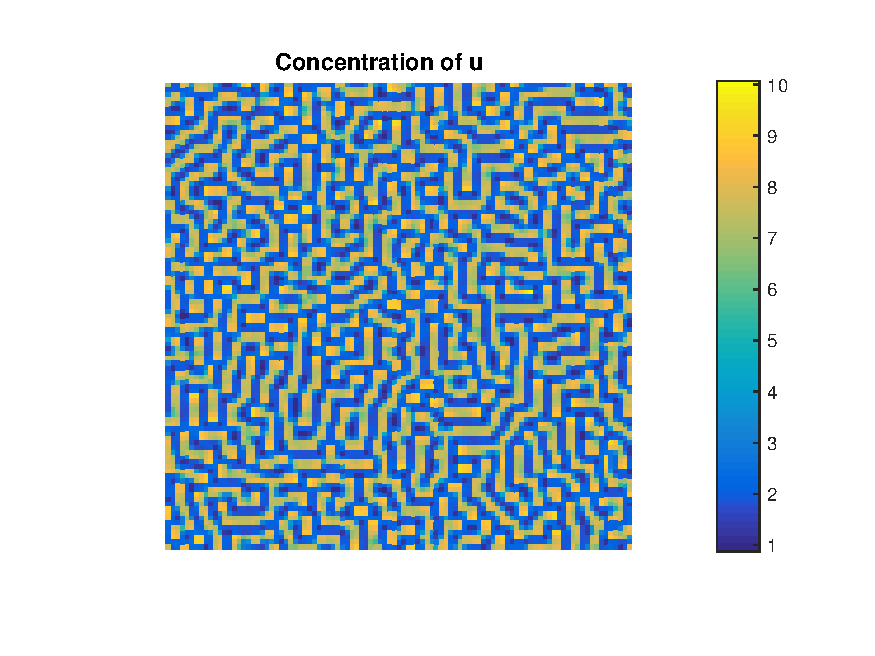
\includegraphics[scale = 0.9]{./plots/cua4p5b9.pdf}
%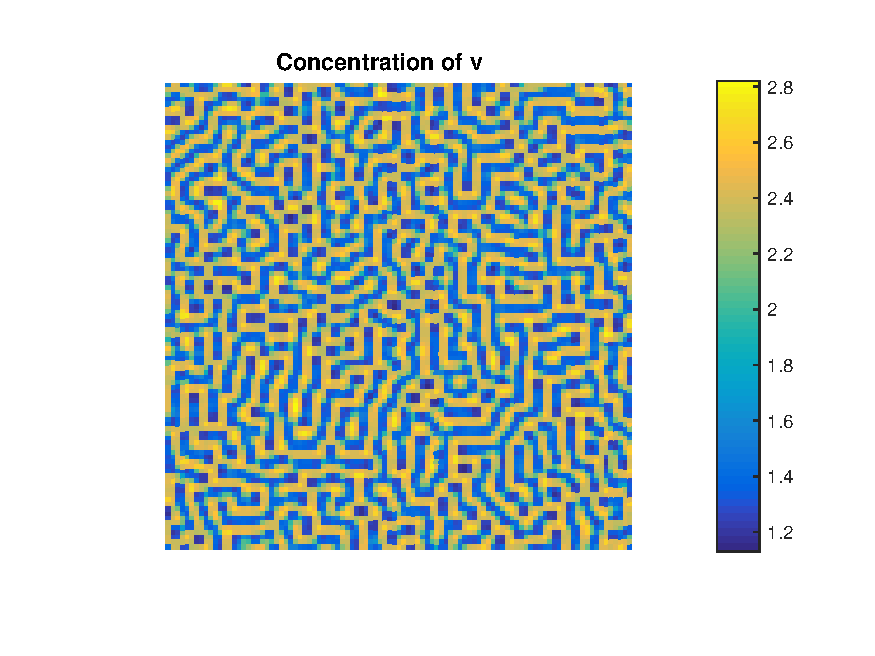
\includegraphics[scale = 0.5]{./plots/cva4p5b9.pdf}
\caption{Brusselator simulation output for $a=4.5,b=9,D_u=1,D_v=8$.}
\label{fig:Brussl2}
\end{figure}



\end{document}
